\documentclass[conference]{IEEEtran}
\IEEEoverridecommandlockouts
% The preceding line is only needed to identify funding in the first footnote. If that is unneeded, please comment it out.
%\usepackage{cite}
\usepackage{amsmath,amssymb,amsfonts}
\usepackage{algorithmic}
\usepackage{graphicx}
\usepackage{subfig}
\usepackage{textcomp}
\usepackage{xcolor}
\def\BibTeX{{\rm B\kern-.05em{\sc i\kern-.025em b}\kern-.08em
    T\kern-.1667em\lower.7ex\hbox{E}\kern-.125emX}}
%% own packages
\usepackage{multirow}
\usepackage{booktabs}
\usepackage[hidelinks]{hyperref}
\usepackage[capitalise]{cleveref}

\usepackage[backend=biber, style=numeric]{biblatex} %Zitate mit BibTeX  %, sorting=none "richtige" Reihenfolge der Nummern
%, citestyle=alphabetic-verb
\bibliography{ML-literature}

\begin{document}

\title{Predicting a vehicles velocity using dashcam footage}

\author{\IEEEauthorblockN{Florian Wolf}
\IEEEauthorblockA{\textit{Department of Mathematics and Statistics, University Konstanz}\\
Konstanz, Germany\\
florian.2.wolf@uni-konstanz.de}
\and
\IEEEauthorblockN{Franz Herbst}
\IEEEauthorblockA{\textit{Department of Physics, University Konstanz} \\
Konstanz, Germany\\
franz.herbst@uni-konstanz.de}
}

\maketitle

\begin{abstract}
In this report bla bla bla
\end{abstract}

\begin{IEEEkeywords}
deep learning, computer vision, visual odometry, dense optical flow, siamese network
\end{IEEEkeywords}

\section{Introduction}
Here are some motivational words needed
\subsection{Aim of the project}
Here we need to clarify the aim of the project and the levels of measurement

ASSUMPTIONS ON MEASUREMENT OF THE RESULTS

ASSUMPTION TRAINING ERROR UNDER 3 IS EXTREMLY GOOD
 

\section{Data collection, analysis and preprocessing}
For our data set, we used the comma ai speedchallenge\footnote{https://github.com/commaai/speedchallenge} data base. This data
set provides two dashcam videos: a training video, (20400 frames, shoot at 20 frames per second) including 
ground truths and a testing video (10798 frames, shoot at 20 frames per second) without labels, which they use for applications 
to check how well a submitted model is able to generalize.
As we only have access to the labels of the test video frames, we decided to split the provided train data by the 80/20 principle into 
training and testing subsets. Here we did not shuffle the data randomly, as we needed to always have two consecutive frames to 
calculate the optical flow. We initially used a hard cut off after 80$\%$ of the frames, as we wanted to test our model on unseen data, 
to measure how good our model is able to generalize. We will analyse this naive approach later, when we take a closer look
at the results.
\subsection{Data analysis}
To analyse the velocity distribution in the two subsets, we plotted the velocity per frame curve in 
\cref{fig:SpeedPerFrameDistributionNewSplitting}. The first 80$\%$ of the video mostly represent highway scenarios 
and the last 20$\%$ only consists of city driving scenes. 
Therefore we did not expect our model to perform really well using the initial splitting, as the models trained and 
tested on totally different road traffic scenarios.

\subsection{Preprocessing}
Each of the provided frames has a size of $(640,480,3)$ pixels. Due to computational limitations, we decided to cut off the last 60 pixels from the lower border, to remove a black frame inside the car, which did not have any effect on the optical flow. Furthermore, we cut the frame size in half and calculated the optical flow using the Farneback pyramid method \cite{Farneback2003} with the following parameters
\begin{align*}
\text{pyramid levels} &:= 3\\
\text{pyramid scaling} &:= 0.5\\
\text{window size} &:= 6\\
\text{pixel neighborhood size} &:= 5\\
\text{SD of the gaussian filter} &:= 1.1
\end{align*}
We choose three pyramid levels, because we wanted the calculations to be more accurate. To decrease the training duration, we halved 
the size of the optical flow frames again, resulting in a resolution of
$(160,105,3)$ pixels per frame. As we used a window size of six pixels, a comparison between the original optical flow and the down 
sampled one lead to the result, that we do not loose a lot of information.

The optical flow calculation returns the magnitude and
the angle of the flow vectors, which we transformed into polar coordinates. To get an RGB image representing the
optical flow of two consecutive frames, we normalized the magnitudes and put them into the third channel of the frame. The values
of the second channel were all set to the value $255$. We then multiplied the angle with the factor $180/(2\pi)$ and set this value 
for the first channel.

We wanted to see, if the model performs better using the dashcam frames as additional material. Therefore, we did the same down 
sampling with the frames.

%\begin{figure}
%\centering
%  \subfloat[Original frame]{\label{figur:1}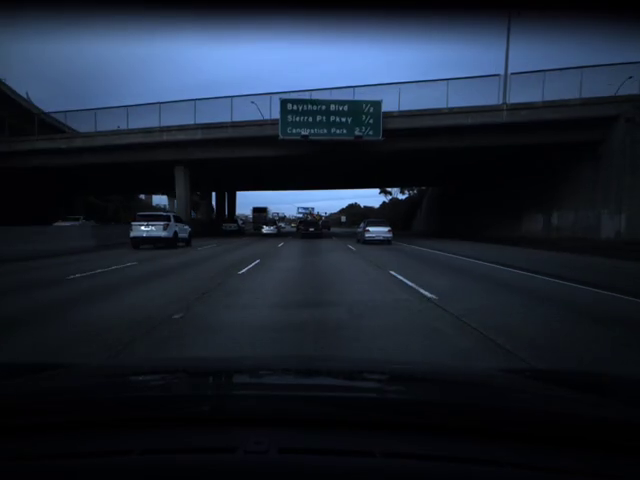
\includegraphics[width=.35\columnwidth]{./imgs/frame2_original.png}} \hspace{0.1cm}
%  \subfloat[Frame after down sampling]{\label{figur:2}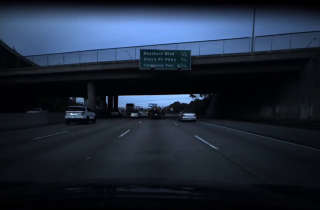
\includegraphics[width=.35\columnwidth]{./imgs/frame2_cut_sampled.png}}\\
%  \subfloat[Optical flow field, already down sampled]{\label{figur:3}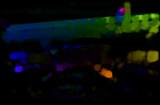
\includegraphics[width=0.7\columnwidth]{./imgs/frame2_flow_field.png}}
%  \label{figur}\caption{Preprocessing of the video frames.}
%\end{figure}

\section{Method selection and architecture}
The prediction of the vehicles speed is a non-linear regression task , so the choice of a neural network is reasonable. 
Recent architectures we discussed in the lecture (ResNet, GoogLeNet, etc.) have shown that using multiple stacked convolution layers
combined with stacked dense layers, perform well on image classification tasks. Therefore the choice of a convolutional neural 
network is justified.

As a performance measure, we choose mean squared errors (MSE).

\subsection{Initial Network}

As an initial architecture we decided to give the model of https://arxiv.org/pdf/1604.07316v1.pdf a try. As the group used it
for self-driving cars, the model has enough complexity to handle a task like ours and with the amount of layers, we had a lot of
possibilities to fine-tune and improve the model.\\
\\HERE SHOULD BE AN IMAGE OF THE NETWORKS ARCHITECTURE\\
\\In a first approach, we tried the raw model gaining an MSE of around 18-20 on testing and under 3 on training. One can clearly 
see, that the model really overfits the train dataset.

\subsection{Siamese approach}

In order to improve our results we expanded our model to also use the original image: Siamese approach

Initial splitting blocks of 100 frames size with 80\% training data, 20\% test data; 20 epochs (train error: 0.411, test error: 2.70)

New splitting: each driving scenario 80\% training data, 20\% test data: (train error: 0.23, test error: 29.7)


\section{Tuning of the model}
To speed up the training we used batch normalization layers https://arxiv.org/pdf/1502.03167.pdf and we tested different activation functions, to improve the performance of the model. 

As proposed in the lecture, we used
\begin{align*}
\mathrm{ReLu}: \mathbb{R} \to \mathbb{R}_0^+, x \mapsto \max\{0,x\}
\end{align*}
as the initial activation function. Using the ReLU function and 15 epochs for training, we achieved a MSE of around 15 on the 
testing set. We ran the 
code multiple times, to ensure this result holds. This result was not really promising, so we wanted to decrease the error by 
modifying the model even more.

As we still had a lot of issues with overfits, we decided to include a dropout layer, according to https://jmlr.org/papers/volume15/srivastava14a/srivastava14a.pdf. We tried different numbers and positions for dropout layers, but using one layer with a dropout 
probability of $p=0.5$ after the third concolutional layer seemed to work best.

To solve the problem of dead neurons\footnote{One can clearly see in the definition of the ReLU 
function, that neurons with a value below zero cannot participate in the learning process.} of the ReLU function, we 
tried the leakyReLU function
\begin{align*}
\mathrm{leakyReLU} : \mathbb{R} \to \mathbb{R}, x \mapsto \begin{cases}
x, x \geq 0\\
c \cdot x, x <0
\end{cases}
\end{align*}
with a hyperparameter $c = 0.01$. Using the leakyReLU function, we achieved a MSE of around 11 on the testing set and under 3 on the 
training set. All of the models were trained with only eight epochs, as we still had problems with overfits.

We identified three possible reasons for our poor results:
\begin{enumerate}
\item[(i)] Too complex model, as the paper used it for autonomous driving or we put too little information into the model.
\item[(ii)] Problems with different brightnesses in the frames (lack of generality), which leads to unstable calculations in the 
optical flow, as the optical flow is quite sensitive to brightness. (Explain how in the train part the sky is quite dark and in the 
city (end) the sky is bright)
\item[(iii)] Too naive/ambigous splitting of the data into train and testing set, as both datasets seem to represent totally different
scenarios in the road traffic.
\end{enumerate}
We came up with the following approaches to solve these problems
\begin{enumerate}
\item[(i)] Simplify the model by using Pooling (we will try average and max pooling), to get more compression and we tried on the
other hand to feed in more information into the model, by using a linear combination of the optical flow and the raw frames itself, and
we tried using a siamese network, to put simultaneously the of and raw frames into the convolutional layers.
\item[(ii)] We wanted to try adding some additional noise into the frames before calculating the optical flow, to make the calculation
more robust against brightness changes. As intentionally adding 
noise to a frame is quite atypical in computer vision, this idea looked quite interesting.
\item[(iii)] Use another splitting. To get a better ratio between highway and city driving scenarios, we decided to split the data into
blocks of 100 frames and take the first 80 for training and the last 20 for testing. Therefore our model should have seen some city
driving.
\end{enumerate}

\subsection{Pooling layers with initial splitting}
We added two generic pooling layers to the network to reduce the number of parameters of the model. One after the second 
convolutional layer and the second one before the fully connected layers start\footnote{Indeed, the number of 
parameters decreased from a total of 636.225 trainable parameters to 156.225. Therefore the number of parameters decreased by a 
factor of 4. We calculated these numbers using the tool pytorch summary.}.We tested maximum and average pooling with the following 
parameters
\begin{align*}
\text{kernel size} &:= 2\times 2\\
\text{stride} &:= 2\\
\text{padding} &:= 1\\
\text{dilatation} &:= \text{None}
\end{align*}
The implementation of pooling layers helped a lot, as now the loss on the train and test data seem to decrease 
nearly equally. Our results on the initial splitting are shown in \cref{tab:ResultsInitialSplitting}. We gave the network
with max pooling a try with 15 epochs, as the loss on the train and test set was decreasing in a pretty stable manner. Using this
network, we achieved for the first time a MSE of under 10 on the test set, which is according to the companies guideline a pretty 
good result --- especially, as we trained the model mostly on highway scenes and tested it only in city driving scenarios.
\begin{table}[!t]
\normalsize
\centering
\begin{tabular}{lcccc}
\toprule
\multirow{2}{*}{Initial splitting, 8 epochs}  & \multicolumn{2}{c}{$\mathrm{ReLU}$} & \multicolumn{2}{c}{$\mathrm{leakyReLU}$} \\
 & Train & Test & Train & Test\\
\midrule
No pooling & 2.85 & 12.08 & 2.45 & 10.75 \\
Max pooling & 5.62 & 11.82 & 5.52 & 10.29 \\
Max pooling (15 epochs) & - & - & \textbf{3.22} & \textbf{9.63} \\
Average pooling & 7.70 & 11.40 & 6.08 & 13.09\\
\bottomrule
\end{tabular}
\caption{MSE results of the network using different pooling strategies, one dropout layers, two different activation functions and 
the initial splitting. We trained each of the models for eight epochs.}
\label{tab:ResultsInitialSplitting}
\end{table}
\subsection{New splitting and siamese network}
We decided to take a closer look at the different road traffic scenarios in the video and segmented the 
frames into three category. The first category
consists of highway driving scenes (from minute 0:00 to minute 7:30), the second one contains frames of 
the car being
in a stop and go scenario on the highway (from minute 7:31 to minute 15:00) and the third category 
consists of
city driving scenes (from minute 15:01 to the end). We visualized the velocity distribution and the 
categories in 
\cref{fig:SpeedPerFrameDistributionNewSplitting}. 
We shuffled the frames of each block randomly and used again the 80/20 rule to split each of the 
category blocks into train and test data.
\begin{figure}[h]
\centering
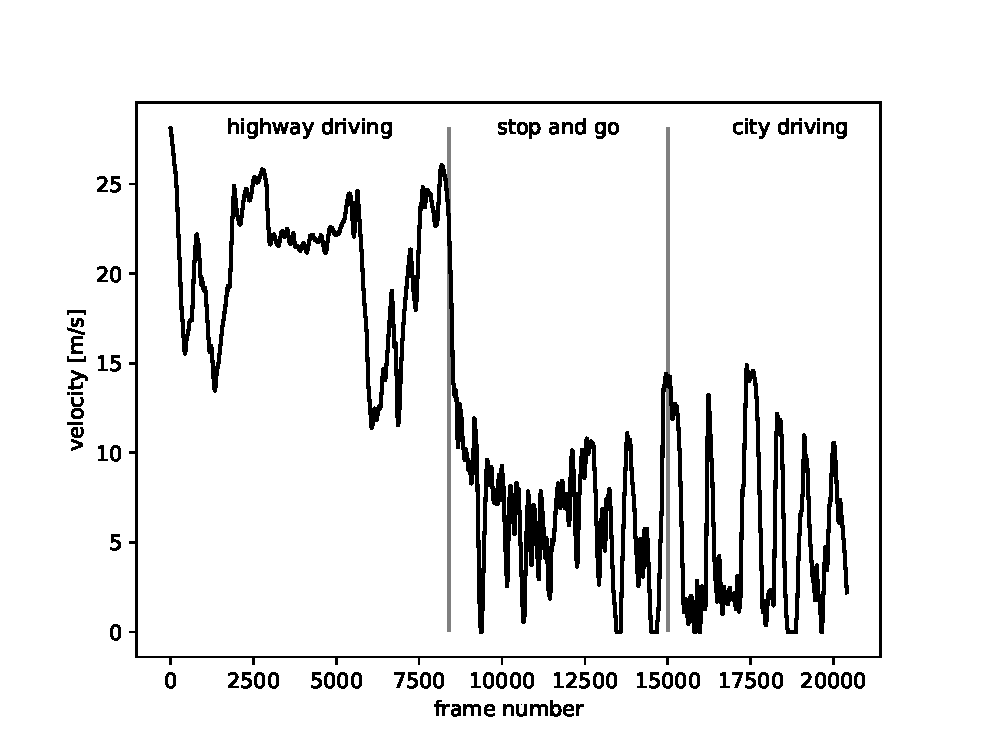
\includegraphics[scale=0.6]{./imgs/plot_speed_time_new_splitting.eps}
\caption{Distribution of the velocities of all frames in the training video including the three categories.}
\label{fig:SpeedPerFrameDistributionNewSplitting}
\end{figure}
\subsection{Augmented brightness}

\section{New Approach using siamese network for two consecutive frames without optical flow}


\section{Error analysis and results}

\section{Further work}

Use MUCH MUCH MUCH MUCH MUCH more data!

Create Validation Data that is not connected to training data and still covers all situations


\section*{Acknowledgment}
We like to thank bla bla bla




\printbibliography


\end{document}
